\documentclass[letterpaper,openany,oneside,twocolumn]{book}

\newcommand{\PATH}{../../}

\usepackage{fontspec}
\usepackage[justified]{\PATH dndtemplate/dnd}
\usepackage{ifthen}
\usepackage{pstricks}

\usepackage{intcalc}

\usepackage[UKenglish]{babel}
\usepackage{\PATH dndtemplate}

\setlength\oddsidemargin{\dimexpr(\paperwidth-\textwidth)/2 - 1in\relax}
\setlength\evensidemargin{\oddsidemargin}

% Headline
\CharacterName{Azriel, Count of Zhalfirim}

\Class{Ranger}
\Level{3}
\Background{Noble}
\PlayerName{M4RZ}
\Race{Vampire}
\Alignment{Lawful Evil}
\XP{}

% Ability scores (correct scores, no modifiers are automatically applied)
% Modifiers, Saving Throws and Skills are calculated automatically
\StrengthScore{15}
\DexterityScore{12}
\ConstitutionScore{17}
\IntelligenceScore{14}
\WisdomScore{16}
\CharismaScore{17}

% Proficiencies (Proficient = 'P', Expertise = 'E', otherwise = '')
\StrengthProficiency{P}
\DexterityProficiency{P}
\ConstitutionProficiency{}
\IntelligenceProficiency{}
\WisdomProficiency{}
\CharismaProficiency{}

\AcrobaticsProficiency{}
\AnimalHandlingProficiency{}
\ArcanaProficiency{}
\AthleticsProficiency{}
\DeceptionProficiency{}
\HistoryProficiency{P}
\InsightProficiency{P}
\IntimidationProficiency{}
\InvestigationProficiency{P}
\MedicineProficiency{}
\NatureProficiency{}
\PerceptionProficiency{P}
\PerformanceProficiency{}
\PersuasionProficiency{P}
\ReligionProficiency{}
\SleightOfHandProficiency{}
\StealthProficiency{}
\SurvivalProficiency{}


\Inspiration{}
\Proficiency{+2}

% Armor Class is not automatically calculated
\ArmorClass{15}
\InitiativeModifier{0}
\Speed{30ft}
\MaxHitPointsRolled{19} % Without Constitution Bonus, is added automatically
\CurrentHitPoints{}
\TemporaryHitPoints{}
\HitDice{d10}
\HitDiceSpent{0}

\CP{}
\SP{}
\EP{}
\GP{225}
\PP{}

% Weapon Arsenal
\AddWeapon{Rapier}{0}{1d8 p}
\AddWeapon{Crossbow}{0}{1d8 p}
\AddWeapon{Claws}{0}{1d6 s}

\AttacksAdditional{
	\textbf{Bite}\\
	\indent 1d6 + \intcalcAdd{\calculateModifier{\StrengthScoreValue}}{0} piercing damage\\\indent\indent + \intcalcAdd{\calculateModifier{\ConstitutionScoreValue}}{0} necrotic damage\\
	\textbf{Rapier of Life Stealing}\\
	\textbf{Crossbow}\\
	\textbf{20 Crossbow Bolts}\\
	\textbf{Armor:} 
	\begin{itemize}
		\item Scale Mail (Stealth Disadvantages)
	\end{itemize}
}

\OtherProficienciesLanguages{
\textbf{Languages:}\\Common, Abyssal, Dwarvish\\
\textbf{Armor:}\\Light Armor, Medium Armor, Shields\\
\textbf{Weapons:}\\Simple Weapons, Martial Weapons\\
\textbf{Tools:}\\Playing Card Set
}

\Equipment{
	a Backpack, a Bedrool, a Mess Kit, a Tinderbox, 10 Torches, 12 Days of Rations, a Waterskin, 50 ft Hempen Rope, a set of fine clothes, a scroll of pedigree \\
	\textbf{Cloak of the Underdark, Crypt Ring}
}

\PersonalityTraits{
	\textbf{Calculating:} Azriel possesses a sharp and strategic mind, carefully considering his actions and weighing their consequences.
}

\Ideals{
	\textbf{Family Legacy:} Azriel's strongest bond lies with the memory of his family and their lost honor, driving his quest for vengeance.
}

\Bonds{
	\textbf{Justice:} Azriel seeks to right the wrongs inflicted upon him and restore justice, both for himself and the innocent.
}

\Flaws{
	\textbf{Dark Desire - Wrath}\\Seeks vengeance against any and all that have wronged them in the most brutal and cruelest fashion.
}

\FeaturesTraits{
\textbf{Vampiric Weakness}
\begin{itemize}
	\item Forbiddance
	\item Running Water
	\item Stake to the Heart
	\item Sunlight Hypersensitivity
\end{itemize}
\textbf{Vampiric Traits (True Vampire)}
\begin{itemize}
	\item Undead
	\item Unholy Body
	\item Blood Connoisseur
	\item Superior Darkvision
	\item Vampire Fangs \& Talons
	\item Misty Escape
\end{itemize}
\textbf{Feats}
\begin{itemize}
	\item Shapechanger (Bat)
	\item Position of Privilege
\end{itemize}
\textbf{Ranger (Swarmkeeper)}
\begin{itemize}
	\item Favored Enemy
	\begin{itemize}
		\item Aberration
	\end{itemize}
	\item Favored Terrain
	\begin{itemize}
		\item Grassland
	\end{itemize}
	\item Fighting Style
	\begin{itemize}
		\item Dueling
	\end{itemize}
	\item Gathered Swarm
	\item Swarmkeeper Magic
	\item Primal Awareness
\end{itemize}
}

% Appearance

\Age{43 (90)}
\Height{6'4}
\Weight{180lbs}
\Eyes{Crimson Red}
\Skin{Pale}
\Hair{Black}

% background

\CharacterAppearance{}{
	\hspace*{-3em}\begin{tabular}{p{90pt}p{80pt}}
		\begin{tabular}{p{90pt}}\vspace*{-0.5em}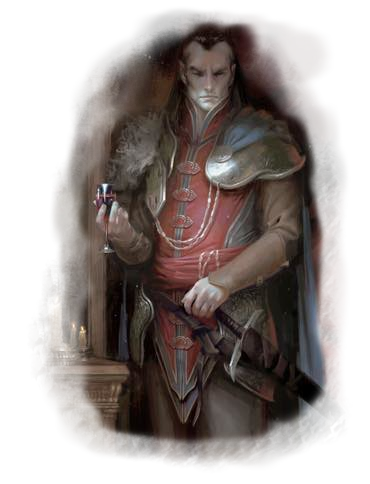
\includegraphics[width=100pt, height=140pt, keepaspectratio]{images/Azriel_appearance.png}\end{tabular}
		&
		\begin{tabular}{p{80pt}}Standing at an imposing height, Azriel, Count of Zhalfirim exudes an aura of undeniable allure and danger. His skin is flawlessly pale, hinting at an eternal existence untouched by the ~~~~~~~~~\end{tabular}
	\end{tabular}\\\vspace*{-1.6em}\hfill\\
	sun's rays. Jet-black, sleek hair cascades down his back, framing a face of sharp, chiseled features. Azriel's eyes, intense and mesmerizing, glow with a piercing crimson hue, reflecting the insatiable thirst for blood.
}{}{}{}
\AdditionalFeaturesAndTraits{
	Azriel's eyes, once vibrant and full of life, have been forever transformed by his vampiric nature. They gleam with an intense, mesmerizing crimson hue, piercing through the darkness with an alluring and magnetic presence. When he locks gazes with others, they feel a strange pull, as if drawn into an enchanting trance.\\
	 Azriel moves with an otherworldly grace, gliding silently and effortlessly through both shadows and crowds. His steps are light and ethereal, leaving barely a whisper as he traverses the realm. There is an enigmatic quality to his presence, an air of elegance and mystery that captivates those around him.\\
	 Azriel's voice is rich and resonant, possessing a velvety quality that carries a subtle hint of allure. When he speaks, it is as if his words are woven into melodic patterns, captivating listeners and leaving them hanging on his every word. His voice carries an innate charm, a subtle manipulation that adds to his influence over others.\\
	As a vampire, Azriel possesses heightened strength, speed, and resilience. His physical prowess surpasses that of mortals, allowing him to overpower opponents with ease. He is also blessed with accelerated healing, quickly recovering from wounds that would prove fatal to others. These supernatural abilities bolster his presence and reinforce his status as a formidable force.
}
\Characterbackground{
	Azriel, once known as Count Azriel of Zhalfirim, led a life of opulence and power as a respected nobleman. However, his idyllic existence shattered when a nefarious rival, Lord Malachi, orchestrated a treacherous coup, accusing Azriel's family of crimes they did not commit. The false allegations led to the downfall of House Zhalfirim, leaving Azriel's loved ones betrayed, imprisoned, or executed.

	Consumed by grief and a burning desire for revenge, Azriel's path led him to the doorstep of a sinister cult. Desperate to avenge his family's honor, he struck a dark bargain with a malevolent entity, willingly sacrificing his humanity to become a vampire and gain the power necessary to enact his revenge.
	
	Azriel's campaign of revenge took him through treacherous lands, navigating dangerous alliances and unearthing long-buried secrets. Along the way, he discovered that Lord Malachi had struck deals with other dark forces, jeopardizing the entire realm. Determined to protect innocent lives, Azriel expanded his vendetta to become a guardian of the realm, purging it of darkness and corruption.
}
\Treasure{
	\textbf{1. The Zhalfirim Family Crest:} A meticulously crafted pendant bearing the emblem of House Zhalfirim. Fashioned from the purest silver, the crest features the regal lion rampant on one side, while the reverse showcases the serene landscape of Zhalfirim. The crest acts as a symbol of Azriel's ancestral lineage and serves as a reminder of the honor and heritage he strives to reclaim.\\
	\textbf{2. The Crypt Ring:} A delicate ring, its band forged from a rare black metal that seems to shimmer with a faint ethereal glow. Nestled within the band is a small, perfectly polished splinter of Azriel's coffinlike structure - the very vessel that held him during his transformation into a vampire. The ring acts as a conduit for his connection to the darkness, granting him a subtle link to his past and serving as a reminder of the sacrifice he made to embark on his path of revenge. When worn, the ring pulses with a faint, otherworldly energy, a constant reminder of his eternal nature and his unyielding determination to reclaim his lost glory.
}
\AlliesAndOrganizations{
	Once a prosperous realm ruled by the esteemed House Zhalfirim, the County of Zhalfirim flourished under the benevolent leadership of Count Azriel. The castle stood as a symbol of grandeur, while the lands thrived with fertile fields and bustling markets. Festivals and celebrations brought joy to the people, and Zhalfirim became renowned for its artisans and scholars. However, shadows crept in as Lord Malachi plotted a coup, accusing House Zhalfirim of crimes. Betrayed and shattered, Zhalfirim fell into darkness. But Count Azriel, driven by vengeance, embraced his transformation into a vampire, determined to restore\linebreak
}{
	his family's honor and reclaim Zhalfirim's prosperity. The stage was set for a battle between light and darkness, shaping the county's fate.
}
\OrganizationName{The County of Zhalfirim}
\OrganizationSymbol{images/Zhalfirim_emblem.png}

% Magic

\SpellcastingClass{Ranger}
\SpellcastingAbility{WIS} % STR, DEX, CON, INT, WIS, CHA
\SpellSaveDCModifier{0} % any modifier that isn't contained in "8 + Ability Modifier + Proficiency Bonus"

\CantripSlotA{Faerie Fire (once per day)}
\CantripSlotB{Mage Hand (once per day)}
\CantripSlotC{Speak with Animals (once per day)}

\FirstLevelSpellSlotsTotal{2}
\FirstLevelSpellSlotA{Detect Poison and Disease}
\FirstLevelSpellSlotB{Fog Cloud}

\begin{document}

\newgeometry{left=0cm,right=0cm,top=0cm,bottom=0cm}
\onecolumn


% CHARACTER PAGE
\rendercharactersheet

% BACKSTORY PAGE
\renderbackgroundsheet

% SPELLCASTING PAGE
\renderspellsheet


\restoregeometry
\twocolumn

\chapter*{Features, Magic Items and Spells}

\section*{Vampire}
\subsection*{Vampiric Weaknesses}
Although vampires can be incredibly strong, their curse still comes with several notable drawbacks. Regardless of if you are a vampire spawn or a true vampire, you are affected by the following weakness unless specified otherwise.
\paragraph*{Forbiddance}
You can't enter a residence without an invitation from one of the occupants.
\paragraph*{Running Water}
Your flesh is torn apart in the presence of water, you take \DndDice{1d12} acid damage when you end your turn in running water. This damage may not be reduced in any way.
\paragraph*{Stake to the Heart}
If a piercing weapon made of wood is driven into your heart while incapacitated in your coffinlike structure, you become paralyzed until the stake is removed if you are a true vampire. However, if you are a vampire spawn, you are instead destroyed.
\paragraph*{Sunlight Hypersensitivity}
You sear and burn in the light of the sun, your flesh immolating. If you end your turn in direct sunlight, you take 20 radiant damage. You also have disadvantage on any attack rolls and ability checks when in direct sunlight.

\subsection*{Vampiric Traits (True Vampire)}
Most of a vampire's victims become vampire spawn, ravenous creatures with a vampire's hunger for blood, but under the control of the vampire that created them. If a true vampire allows a spawn to draw blood from its own body, the spawn transforms into a true vampire no longer under its master's control. Few vampires are willing to relinquish their control in this manner. A vampire spawn becomes free-willed when their creator dies but may seek to become true vampires via drinking from another true vampire or making a pact with some otherworldly entity.
\paragraph*{Undead}
Your creature type is considered to be both humanoid and undead.
\paragraph*{Unholy Body}
Dark magic sustains you, making you resistant to necrotic damage. Healing potions do not have a healing effect on you. Instead, they deal poison damage equal to the amount that was meant to heal. To heal you must either drink blood, spend hit dice, or finish a long rest.
\paragraph*{Blood Connoisseur}
Even though you are undead, you still require sustenance in the form of blood to sustain your unholy existence. You are immune to diseases. You do not need to eat or breathe, but you can ingest food and drink if you wish, though this food is always bland and stale to you. If you go for longer then seven days without drinking at least one ration of blood, at the midnight of the seventh day and every midnight on days thereafter, you suffer one level of exhaustion, which can only be removed by drinking a ration of blood. After consuming one ration of blood, you recover all levels of exhaustion caused by this trait. If you reach 6 levels of exhaustion due to this trait, instead of suffering death, no longer gain any more levels of exhaustion and become indefinitely paralyzed. The only way to remove this paralyze is to be exposed to a rations worth of blood.

A ration of blood is a vial, or 4 ounces, and while that is just enough to sustain you each week, you still feel the urge to drink and may still appear twitchy or ravenous in the heat of battle or when treating a wounded ally. A pint, such as that contained within a flask is considered a healthy amount, enough to keep you sustained while also suppressing your less civilized behavior. Each ration of blood heals you for \DndDice{1d4 + 1} hit points while a pint will heal you for \DndDice{2d4 + 2} hit points.
\paragraph*{Superior Darkvision}
You can see in dim light within 120 feet of you as if it were bright light, and in darkness as if it were dim light. You can't discern color in darkness, only shades of gray.
\paragraph*{Vampire Fangs \& Talons}
All vampires have sharpened teeth capable of tearing flesh from bone and draining blood from the body and elongated claws, their natural weapon, which can be used to make an unarmed strike.
\subparagraph*{Bite}
If a willing, paralyzed, charmed, incapacitated, restrained, or grappled, creature within 5 feet of you has blood, you may use your bonus action to Bite them dealing \DndDice{1d6} piercing damage and draining their blood dealing additional necrotic damage equal to your Constitution modifier (minimum 1 necrotic damage). Drinking blood this way is equal to consuming a ration as per your Blood Connoisseur trait. If this trait fails to deal at least one point of necrotic damage, you also fail to drink any blood. The damage for your Bite increases by 1d6 when you reach 5th level (2d6), 11th level (3d6), and 17th level (4d6).
\subparagraph*{Claws}
You may use your Strength or Dexterity modifier for your attack and damage rolls with your claws. If you hit with them, you deal \DndDice{1d6} slashing damage instead of the bludgeoning damage normal for an unarmed strike.\\
\paragraph*{Misty Escape}
When you drop to 0 hit points outside of your coffinlike structure, you transform into a cloud of mist instead of falling unconscious, provided you are not in an area of sunlight or running water. If you can't transform, you are destroyed.

While in mist form, you can't take any actions, speak, or manipulate objects. You are weightless, have a flying speed of 20 feet, can hover, and can enter a hostile creature's space and stop there. In addition, if air can pass through a space, the mist can do so without squeezing, and it can't pass through water. It has advantage on Strength, Dexterity, and Constitution saving throws, and is immune to all nonmagical damage, except the damage it takes from sunlight.

While you have 0 hit points in mist form, you can't revert to your vampire form. If you do not reach your coffinlike structure within 2 hours, you are destroyed. Once in your coffinlike structure, you revert to your vampire form. You are then paralyzed until you regain at least 1 hit point. After spending 1 hour in your coffinlike structure with 0 hit points, you regain 1 hit point.

\section*{Ranger}
\subsection*{Favored Enemy}
You have significant experience studying, tracking, hunting, and even talking to a certain type of enemy.

Choose a type of favored enemy: aberrations, beasts, celestials, constructs, dragons, elementals, fey, fiends, giants, monstrosities, oozes, plants, or undead. Alternatively, you can select two races of humanoid (such as gnolls and orcs) as favored enemies.

You have advantage on Wisdom (Survival) checks to track your favored enemies, as well as on Intelligence checks to recall information about them.

When you gain this feature, you also learn one language of your choice that is spoken by your favored enemies, if they speak one at all.

You choose one additional favored enemy, as well as an associated language, at 6th and 14th level. As you gain levels, your choices should reflect the types of monsters you have encountered on your adventures.

\subsection*{Natural Explorer}
You are particularly familiar with one type of natural environment and are adept at traveling and surviving in such regions. Choose one type of favored terrain: arctic, coast, desert, forest, grassland, mountain, swamp, or the Underdark. When you make an Intelligence or Wisdom check related to your favored terrain, your proficiency bonus is doubled if you are using a skill that you're proficient in.

While traveling for an hour or more in your favored terrain, you gain the following benefits:
\begin{itemize}
	\item Difficult terrain doesn't slow your group's travel.
	\item Your group can't become lost except by magical means.
	\item Even when you are engaged in another activity while traveling (such as foraging, navigating, or tracking), you remain alert to danger.
	\item If you are traveling alone, you can move stealthily at a normal pace.
	\item When you forage, you find twice as much food as you normally would.
	\item While tracking other creatures, you also learn their exact number, their sizes, and how long ago they passed through the area.
\end{itemize}
You choose additional favored terrain types at 6th and 10th level.

\subsection*{Fighting Style}
You adopt a particular style of fighting as your specialty. Choose one of the following options.

You can't take a Fighting Style option more than once, even if you later get to choose again.

\subsubsection*{Dueling}
When you are wielding a melee or martial weapon in one hand and no other weapons, you gain a +2 bonus to damage rolls with that weapon.

\subsection*{Ranger Archetypes}
\subsubsection*{Swarmkeeper}
\paragraph*{Gathered Swarm}
At 3rd level, a swarm of intangible nature spirits has bonded itself to you and can assist you in battle. Until you die, the swarm remains in your space, crawling on you or flying and skittering around you within your space. Because of your vampiric nature these nature spirits have taken the form of bats.\\
Once on each of your turns, you can cause the swarm to assist you in one of the following ways, immediately after you hit a creature with an attack:
\begin{itemize}
	\item The attack's target takes \DndDice{1d6} piercing damage from the swarm.
	\item The attack's target must succeed on a Strength saving throw against your spell save DC or be moved by the swarm up to 15 feet horizontally in a direction of your choice.
	\item You are moved by the swarm 5 feet horizontally in a direction of your choice.
\end{itemize}
\paragraph*{Swarmkeeper Magic}
Also at 3rd level, you learn the Mage Hand cantrip if you don't already know it. When you cast it, the hand takes the form of your swarming nature spirits.\\
You also learn an additional spell of 1st level or higher when you reach certain levels in this class, as shown in the Swarmkeeper Spells table. Each spell counts as a ranger spell for you, but it doesn't count against the number of ranger spells you know.
\begin{DndTable}[header=Swarmkeeper Spells]{lXX}
			& Ranger Level 	& Spell						\\
$\bullet$ 	& 3rd 			& Faerie Fire, Mage Hand		\\
			& 5th 			& Web						\\
			& 9th 			& Gaseous Form				\\
			& 13th 			& Arcane Eye					\\
			& 17th 			& Insect Plague				\\
\end{DndTable}

\subsection*{Primal Awareness}
You can focus your awareness through the interconnections of nature learning additional spells when you reach certain levels in this class, as shown in the Primal Awareness Spells table. These spells don't count against the number of ranger spells you know.
\begin{DndTable}[header=Primal Awareness Spells]{lXX}
			& Ranger Level 	& Spell						\\
$\bullet$ 	& 3rd 			& Speak with Animals		\\
			& 5th 			& Beast Sense				\\
			& 9th 			& Speak with Plants			\\
			& 13th 			& Locate Creature			\\
			& 17th 			& Commune with Nature		\\
\end{DndTable}
Once per long rest, you can cast each of these spells once without expending a spell slot.

\section*{Feats}
\subsection*{Shapechanger (Bat)}
Vampires are known for their ability to shift from form to form. You gain the shapechanger tag and if you are not in sunlight or running water, you can use your action to polymorph into a Tiny bat[1] or a Medium cloud of mist for 1 minute, or back into your true form.
\paragraph*{Bat Form}
While in bat form you can't speak, your walking speed is 5 feet, and you have a flying speed of 30 feet. Your statistics, other than your size and speed, are unchanged. Anything you are wearing transforms with you, but nothing you are carrying does. You revert to your true form if you die.\\
Once you transform this way you cannot do so again until you complete a short or long rest.
\subsection*{Position of Privilege}
Thanks to your noble birth, people are inclined to think the best of you. You are welcome in high society, and people assume you have the right to be wherever you are. The common folk make every effort to accommodate you and avoid your displeasure, and other people of high birth treat you as a member of the same social sphere. You can secure an audience with a local noble if you need to.

\section*{Magical Items}
\subsection*{Rapier of Life Stealing}
When you attack a creature with this magic weapon and roll a 20 on the attack roll, that target takes an extra 10 necrotic damage if it isn't a construct or an undead. You also gain 10 temporary hit points.
\subsection*{Cloak of the Underdark}
\textit{Wondrous item, uncommon (requires attunement)}

This exotic garment of drow design is made of black silk interwoven with faint silver threads. While wearing this cloak, you can pull its hood over your head to cause yourself to become immune to the effects of sunlight. The cloak allows for no sunlight to pass through.
\subsection*{Crypt Ring}
\textit{Ring, very rare (requires attunement)}

This ring can only be attuned by a true vampire. It holds a small compartment in its silver head, containing a small part of your coffinlike structure such as a piece of stonework, a chunk of wood, or compressed dirt. While worn with a part of your coffinlike structure is placed here, any coffinlike structure has the same effect as your coffinlike structure.

\section*{Spells}
\subsection*{Cantrip}

\DndSpellHeader
  {Faerie Fire}
  {1st-Level Evocation}
  {1 Action}
  {60 feet}
  {V}
  {Concentration, up to 1 minute}

Each object in a 20-foot cube within range is outlined in blue, green, or violet light (your choice). Any creature in the area when the spell is cast is also outlined in light if it fails a Dexterity saving throw. For the duration, objects and affected creatures shed dim light in a 10-foot radius.

Any attack roll against an affected creature or object has advantage if the attacker can see it, and the affected creature or object can't benefit from being invisible.

\DndSpellHeader
  {Mage Hand}
  {Conjuration Cnatrip}
  {1 Action}
  {30 feet}
  {V, S}
  {1 minute}

A spectral, floating hand appears at a point you choose within range. The hand lasts for the duration or until you dismiss it as an action. The hand vanishes if it is more than 30 feet away from you or if you cast this spell again.

You can use your action to control the hand. You can use the hand to manipulate an object, open an unlocked door or container, stow or retrieve an item from an open container, or pour the contents out of a vial. You can move the hand up to 30 feet each time you use it.

The hand can't attack, activate magic items, or carry more than 10 pounds.

\DndSpellHeader
  {Speak with Animals}
  {1st-Level Divination (Ritual)}
  {1 Action}
  {Self}
  {V, S}
  {10 minutes}

You gain the ability to comprehend and verbally communicate with beasts for the duration. The knowledge and awareness of many beasts is limited by their intelligence, but at minimum, beasts can give you information about nearby locations and monsters, including whatever they can perceive or have perceived within the past day. You might be able to persuade a beast to perform a small favor for you, at the DM's discretion.

\subsection*{Level 1}

\DndSpellHeader
  {Detect Poison and Disease}
  {1st-Level Divination (Ritual)}
  {1 Action}
  {Self}
  {V, S}
  {Concentration, up to 10 minutes}

For the duration, you can sense the presence and location of poisons, poisonous creatures, and diseases within 30 feet of you. You also identify the kind of poison, poisonous creature, or disease in each case.

The spell can penetrate most barriers, but it is blocked by 1 foot of stone, 1 inch of common metal, a thin sheet of lead, or 3 feet of wood or dirt.

\hfill\\

\DndSpellHeader
  {Fog Cloud}
  {1st-Level Conjuration}
  {1 Action}
  {120 feet}
  {V, S}
  {Concentration, up to 1 hour}

You create a 20-foot-radius sphere of fog centered on a point within range. The sphere spreads around corners, and its area is heavily obscured. It lasts for the duration or until a wind of moderate or greater speed (at least 10 miles per hour) disperses it

\subparagraph*{At Higher Levels} When you cast this spell using a spell slot of 2nd level or higher, the radius of the fog increases by 20 feet for each slot level above 1st.

\section*{Miscellaneous}
\subsection*{Attack and Damage Rolls}
\subsubsection*{Martial Weapon}
\paragraph*{Attack Roll}\hfill\\
\underline{Rapier of Life Stealing:}\\
1d20 + DEX-Modifier + Proficiency Modifier\\
\indent Current Max: \intcalcAdd{20}{\intcalcAdd{\calculateModifier{\DexterityScoreValue}}{\ProficiencyValue}}
\paragraph*{Damage Roll}\hfill\\
\underline{Rapier of Life Stealing:}\\
1d8 + DEX-Modifier + 2 (Fighting Style: Dueling) (+ 10 Life Steal if Hit-Dice 20)\\
\indent Current Max (Normal): \intcalcAdd{8}{\intcalcAdd{\calculateModifier{\DexterityScoreValue}}{2}}\\
\indent Current Max (Life Steal): \intcalcAdd{8}{\intcalcAdd{\calculateModifier{\DexterityScoreValue}}{\intcalcAdd{2}{10}}}
\subsubsection*{Ranged Weapon}
\paragraph*{Attack Roll}\hfill\\
\underline{Crossbow:}\\
1d20 + DEX-Modifier + Proficiency Modifier\\
\indent Current Max: \intcalcAdd{20}{\intcalcAdd{\calculateModifier{\DexterityScoreValue}}{\ProficiencyValue}}
\paragraph*{Damage Roll}\hfill\\
\underline{Crossbow:}\\
1d8 + DEX-Modifier\\
\indent Current Max (Normal): \intcalcAdd{8}{\calculateModifier{\DexterityScoreValue}}
\subsubsection*{Vampiric Attacks}
\paragraph*{Attack Roll}\hfill\\
\underline{Bite:}\\
1d20 + STR-Modifier + Proficiency Modifier\\
\indent Current Max: \intcalcAdd{20}{\intcalcAdd{\calculateModifier{\StrengthScoreValue}}{\ProficiencyValue}}\\
\underline{Claw:}\\
1d20 + STR-Modifier + Proficiency Modifier\\
\indent Current Max: \intcalcAdd{20}{\intcalcAdd{\calculateModifier{\StrengthScoreValue}}{\ProficiencyValue}}
\paragraph*{Damage Roll}\hfill\\
\underline{Bite:}\\
1d6 + STR-Modifier + CON-Modifier\\
\indent Current Max: \intcalcAdd{6}{\calculateModifier{\StrengthScoreValue}} piercing + \intcalcAdd{\calculateModifier{\ConstitutionScoreValue}}{0} necrotic damage\\
\underline{Claw:}\\
1d6 + STR-Modifier\\
\indent Current Max: \intcalcAdd{6}{\calculateModifier{\StrengthScoreValue}}

\end{document}
